%%%%%%%%%%%%%%%%%%%%%%%%%%%%%%%%%%%%%%%%%%%%%%%%%%%%%%%%%%%%%%%%%%%%%%%%%%%%%%%%
%2345678901234567890123456789012345678901234567890123456789012345678901234567890
%        1         2         3         4         5         6         7         8

\documentclass[letterpaper, 10 pt, conference]{ieeeconf}  % Comment this line out if you need a4paper
\usepackage{amsmath, xparse}
\usepackage{amstext}
\usepackage{amsfonts}
\usepackage{float}
\usepackage{graphicx}

%\documentclass[a4paper, 10pt, conference]{ieeeconf}      % Use this line for a4 paper

\IEEEoverridecommandlockouts                              % This command is only needed if
                                                          % you want to use the \thanks command

\overrideIEEEmargins                                      % Needed to meet printer requirements.

%In case you encounter the following error:
%Error 1010 The PDF file may be corrupt (unable to open PDF file) OR
%Error 1000 An error occurred while parsing a contents stream. Unable to analyze the PDF file.
%This is a known problem with pdfLaTeX conversion filter. The file cannot be opened with acrobat reader
%Please use one of the alternatives below to circumvent this error by uncommenting one or the other
%\pdfobjcompresslevel=0
%\pdfminorversion=4

% See the \addtolength command later in the file to balance the column lengths
% on the last page of the document

% The following packages can be found on http:\\www.ctan.org
%\usepackage{graphics} % for pdf, bitmapped graphics files
%\usepackage{epsfig} % for postscript graphics files
%\usepackage{mathptmx} % assumes new font selection scheme installed
%\usepackage{times} % assumes new font selection scheme installed
%\usepackage{amsmath} % assumes amsmath package installed
%\usepackage{amssymb}  % assumes amsmath package installed

\title{\LARGE \bf
Homework 2 Report
}


\author{Arrian Chi% <-this % stops a space
}


\begin{document}

\onecolumn


\maketitle
\thispagestyle{empty}
\pagestyle{empty}


%%%%%%%%%%%%%%%%%%%%%%%%%%%%%%%%%%%%%%%%%%%%%%%%%%%%%%%%%%%%%%%%%%%%%%%%%%%%%%%%

\begin{abstract}

In this homework, I reviewed the concepts of linear and nonlinear regression and applied them to the data set. 

\end{abstract}

\section*{Problem 1}
\subsection*{a:}
\begin{figure}[!ht]
        \centering
        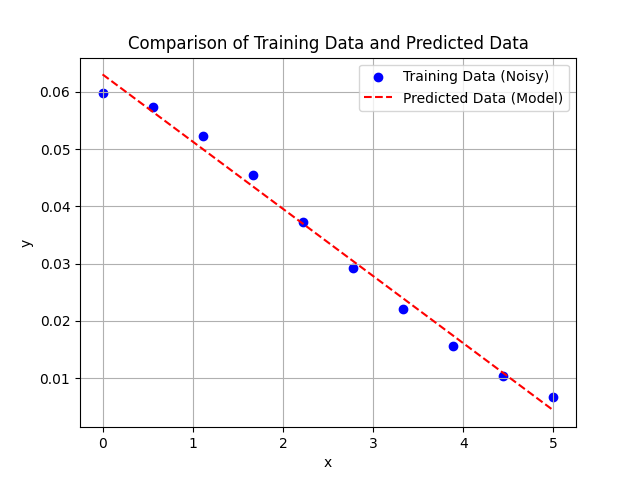
\includegraphics[width=0.7\textwidth,keepaspectratio]{linear_fit.png}
        \caption{Plot of predicted values of $y_{pred}$ versus actual values of $y_{actual}$ (linear)}
        \label{fig:linear_fit}
\end{figure}
\subsection*{b:}
The number of epochs is the number of times the gradient descent will be applied, while the learning rate controls how much the prediction changes at each step. Increasing the number of epochs will slow down the performance of the model (takes more time to iterate) while increasing the learning rate will make the model step faster. However if the learning rate is too high, the model may become unstable and not converge. If the learning rate is too low (relative to epochs), the model may take a long time to converge and still not have converged at the end of the operation. If the epochs is too high, it is possible that the model will overfit the data or do redundant fitting, but if the epochs is too low, the model may not have enough time to converge.

The best combination that minimizes loss the quickest with a final $\text{loss} = 0.0000034267728104$ are $\text{epochs} = 1000$ and $\text{learning\_rate} = 0.1$. Even for smaller learning rates and larger numbers of epochs, the model converges to this final loss (it can't get any better). 


\clearpage

\section*{Problem 2}
\subsection*{a:}
\begin{figure}[!ht]
        \centering
        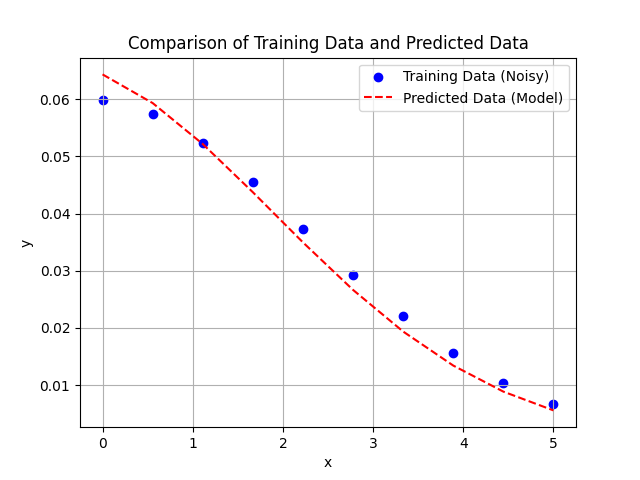
\includegraphics[width=0.7\textwidth,keepaspectratio]{nonlinear_fit.png}
        \caption{Plot of predicted values of $y_{pred}$ versus actual values of $y_{actual}$ (nonlinear)}
        \label{fig:nonlinear_fit}
\end{figure}
\subsection*{b:}
The previous section about epochs and learning rates is applicable, however I found that if the epochs or the learning rate is too high, the model will start diverging (we see the loss increasing/we start seeing NaNs!). I also found that a good initial guess for the parameters is important for the model to converge because it is possible for the model to converge onto local minima. Algorithms like simulated annealing could help minimize the chance of this happening (finding the global minimum).

The best combination that minimizes loss with a final $\text{loss} = 0.000005445874$ are $\text{epochs} = 96200$ and $\text{learning\_rate} = 0.0001$. Beyond this, the model starts diverging (stepping away from this minima).
% \begin{figure}[!ht]
%         \centering
%         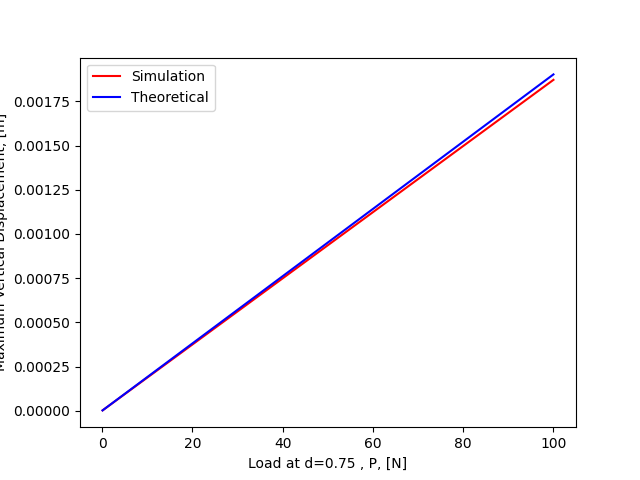
\includegraphics[width=0.45\textwidth,keepaspectratio]{p3_implicit_maxvert2xzoomed.png}
%         \caption{Plot of Maximum Vertical Displacement of the Beam v.s. the size of the point load (zoomed in again)}
%         \label{"fig:p3q2_benefit_zoomed2x"}
% \end{figure}

\addtolength{\textheight}{-12cm}   % This command serves to balance the column lengths
                                  % on the last page of the document manually. It shortens
                                  % the textheight of the last page by a suitable amount.
                                  % This command does not take effect until the next page
                                  % so it should come on the page before the last. Make
                                  % sure that you do not shorten the textheight too much.

%%%%%%%%%%%%%%%%%%%%%%%%%%%%%%%%%%%%%%%%%%%%%%%%%%%%%%%%%%%%%%%%%%%%%%%%%%%%%%%%



%%%%%%%%%%%%%%%%%%%%%%%%%%%%%%%%%%%%%%%%%%%%%%%%%%%%%%%%%%%%%%%%%%%%%%%%%%%%%%%%



\end{document}
